Así como se pueden agregar agentes nuevos, también pueden ser eliminados, es por esto que para eliminar un agente, se implemento una funcionalidad muy sencilla. Como se observa en la figura \ref{image:eliminarCompleto}, tenemos nuestra pantalla principal y a lado de cada agente se observa 3 botones que corresponden a la visualización de las gráficas, de la información de cada agente y a la eliminación del mismo. La figura \ref{image:botones} muestra más de cerca los botones mencionados anteriormente.

\FloatBarrier
\begin{figure}[htbp!]
		\centering
	\includegraphics[width=1.1 \textwidth]{images/eliminarCompleto}
		\caption{Pantalla de inicio que muestra botón para eliminar un agente.}		\label{image:eliminarCompleto}
\end{figure}
\FloatBarrier

\FloatBarrier
\begin{figure}[htbp!]
		\centering
	\includegraphics[width=.3 \textwidth]{images/botones}
		\caption{Botones de pantalla de principal.}		\label{image:botones}
\end{figure}
\FloatBarrier

El código para la funcionalidad de esta parte es el mostrado en la figura \ref{image:eliminar}, en el cual al presionar dicho botón, se habla al método eliminarAgente enviando como parámetro la ip del agente a eliminar, lo que realiza este método es, nuevamente recorrer nuestro archivo hosts e ir guardando en un arreglo todo lo que lee de dicho archivo, en caso de que encuentre la ip que recibió como parámetro, no guarda esa línea de información y posteriormente sobreescribe el archivo con toda la información del arreglo. En otras palabras, sobreescribe el archivo sin la línea del agente que se eliminó.
\FloatBarrier
\begin{figure}[htbp!]
		\centering
	\includegraphics[width=.5 \textwidth]{images/eliminar}
		\caption{Método eliminarAgente.}		\label{image:eliminar}
\end{figure}
\FloatBarrier

Después de que se ha ejecutado este método, aparece una pequeña alerta como la de la figura \ref{image:alertaE} donde se muestra que nuestro agente ha sido eliminado y se llama al método main (figura \ref{image:main} el cual como se observa, llama al método getHostInfo y se repite todo el procedimiento explicado en la sección "Pantalla de inicio".

\FloatBarrier
\begin{figure}[htbp!]
		\centering
	\includegraphics[width=.4 \textwidth]{images/alertaE}
		\caption{Alerta de agente eliminado.}		\label{image:alertaE}
\end{figure}
\FloatBarrier

\FloatBarrier
\begin{figure}[htbp!]
		\centering
	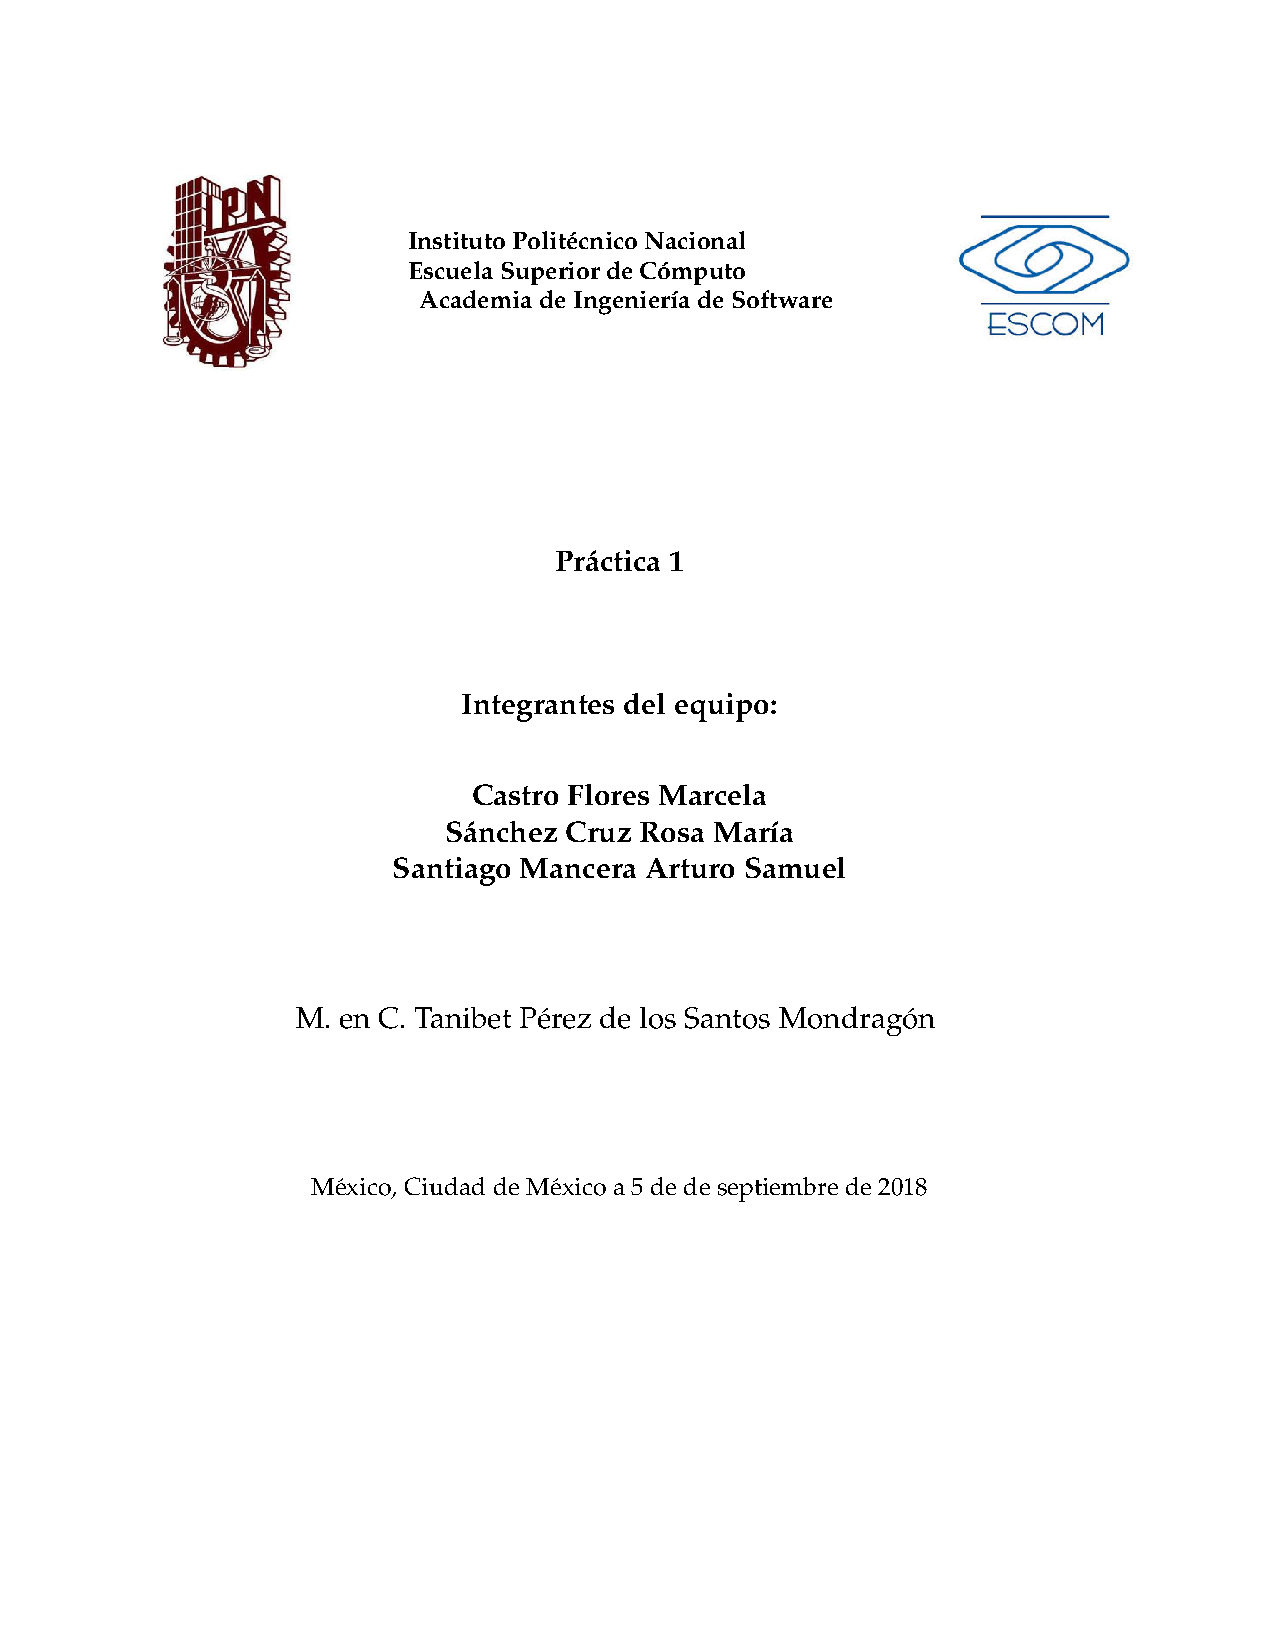
\includegraphics[width=.4 \textwidth]{images/main}
		\caption{Método main.}		\label{image:main}
\end{figure}
\FloatBarrier

Nuevamente se recarga la pantalla principal para observar que la información de nuestro agente ya no se plasma en esta (figura \ref{image:principalSA}) ni tampoco en nuestro archivo de hosts (figura \ref{image:hostsSA}).

\FloatBarrier
\begin{figure}[htbp!]
		\centering
	\includegraphics[width=1.1 \textwidth]{images/principalSA}
		\caption{Pantalla principal sin el agente eliminado.}		\label{image:principalSA}
\end{figure}
\FloatBarrier

\FloatBarrier
\begin{figure}[htbp!]
		\centering
	\includegraphics[width=.6 \textwidth]{images/hostsSA}
		\caption{Archivo hosts sin el agente eliminado.}		\label{image:hostsSA}
\end{figure}
\FloatBarrier